\begin{frame}
  \frametitle{The necessity of manipulation-based search}
  \begin{center}
    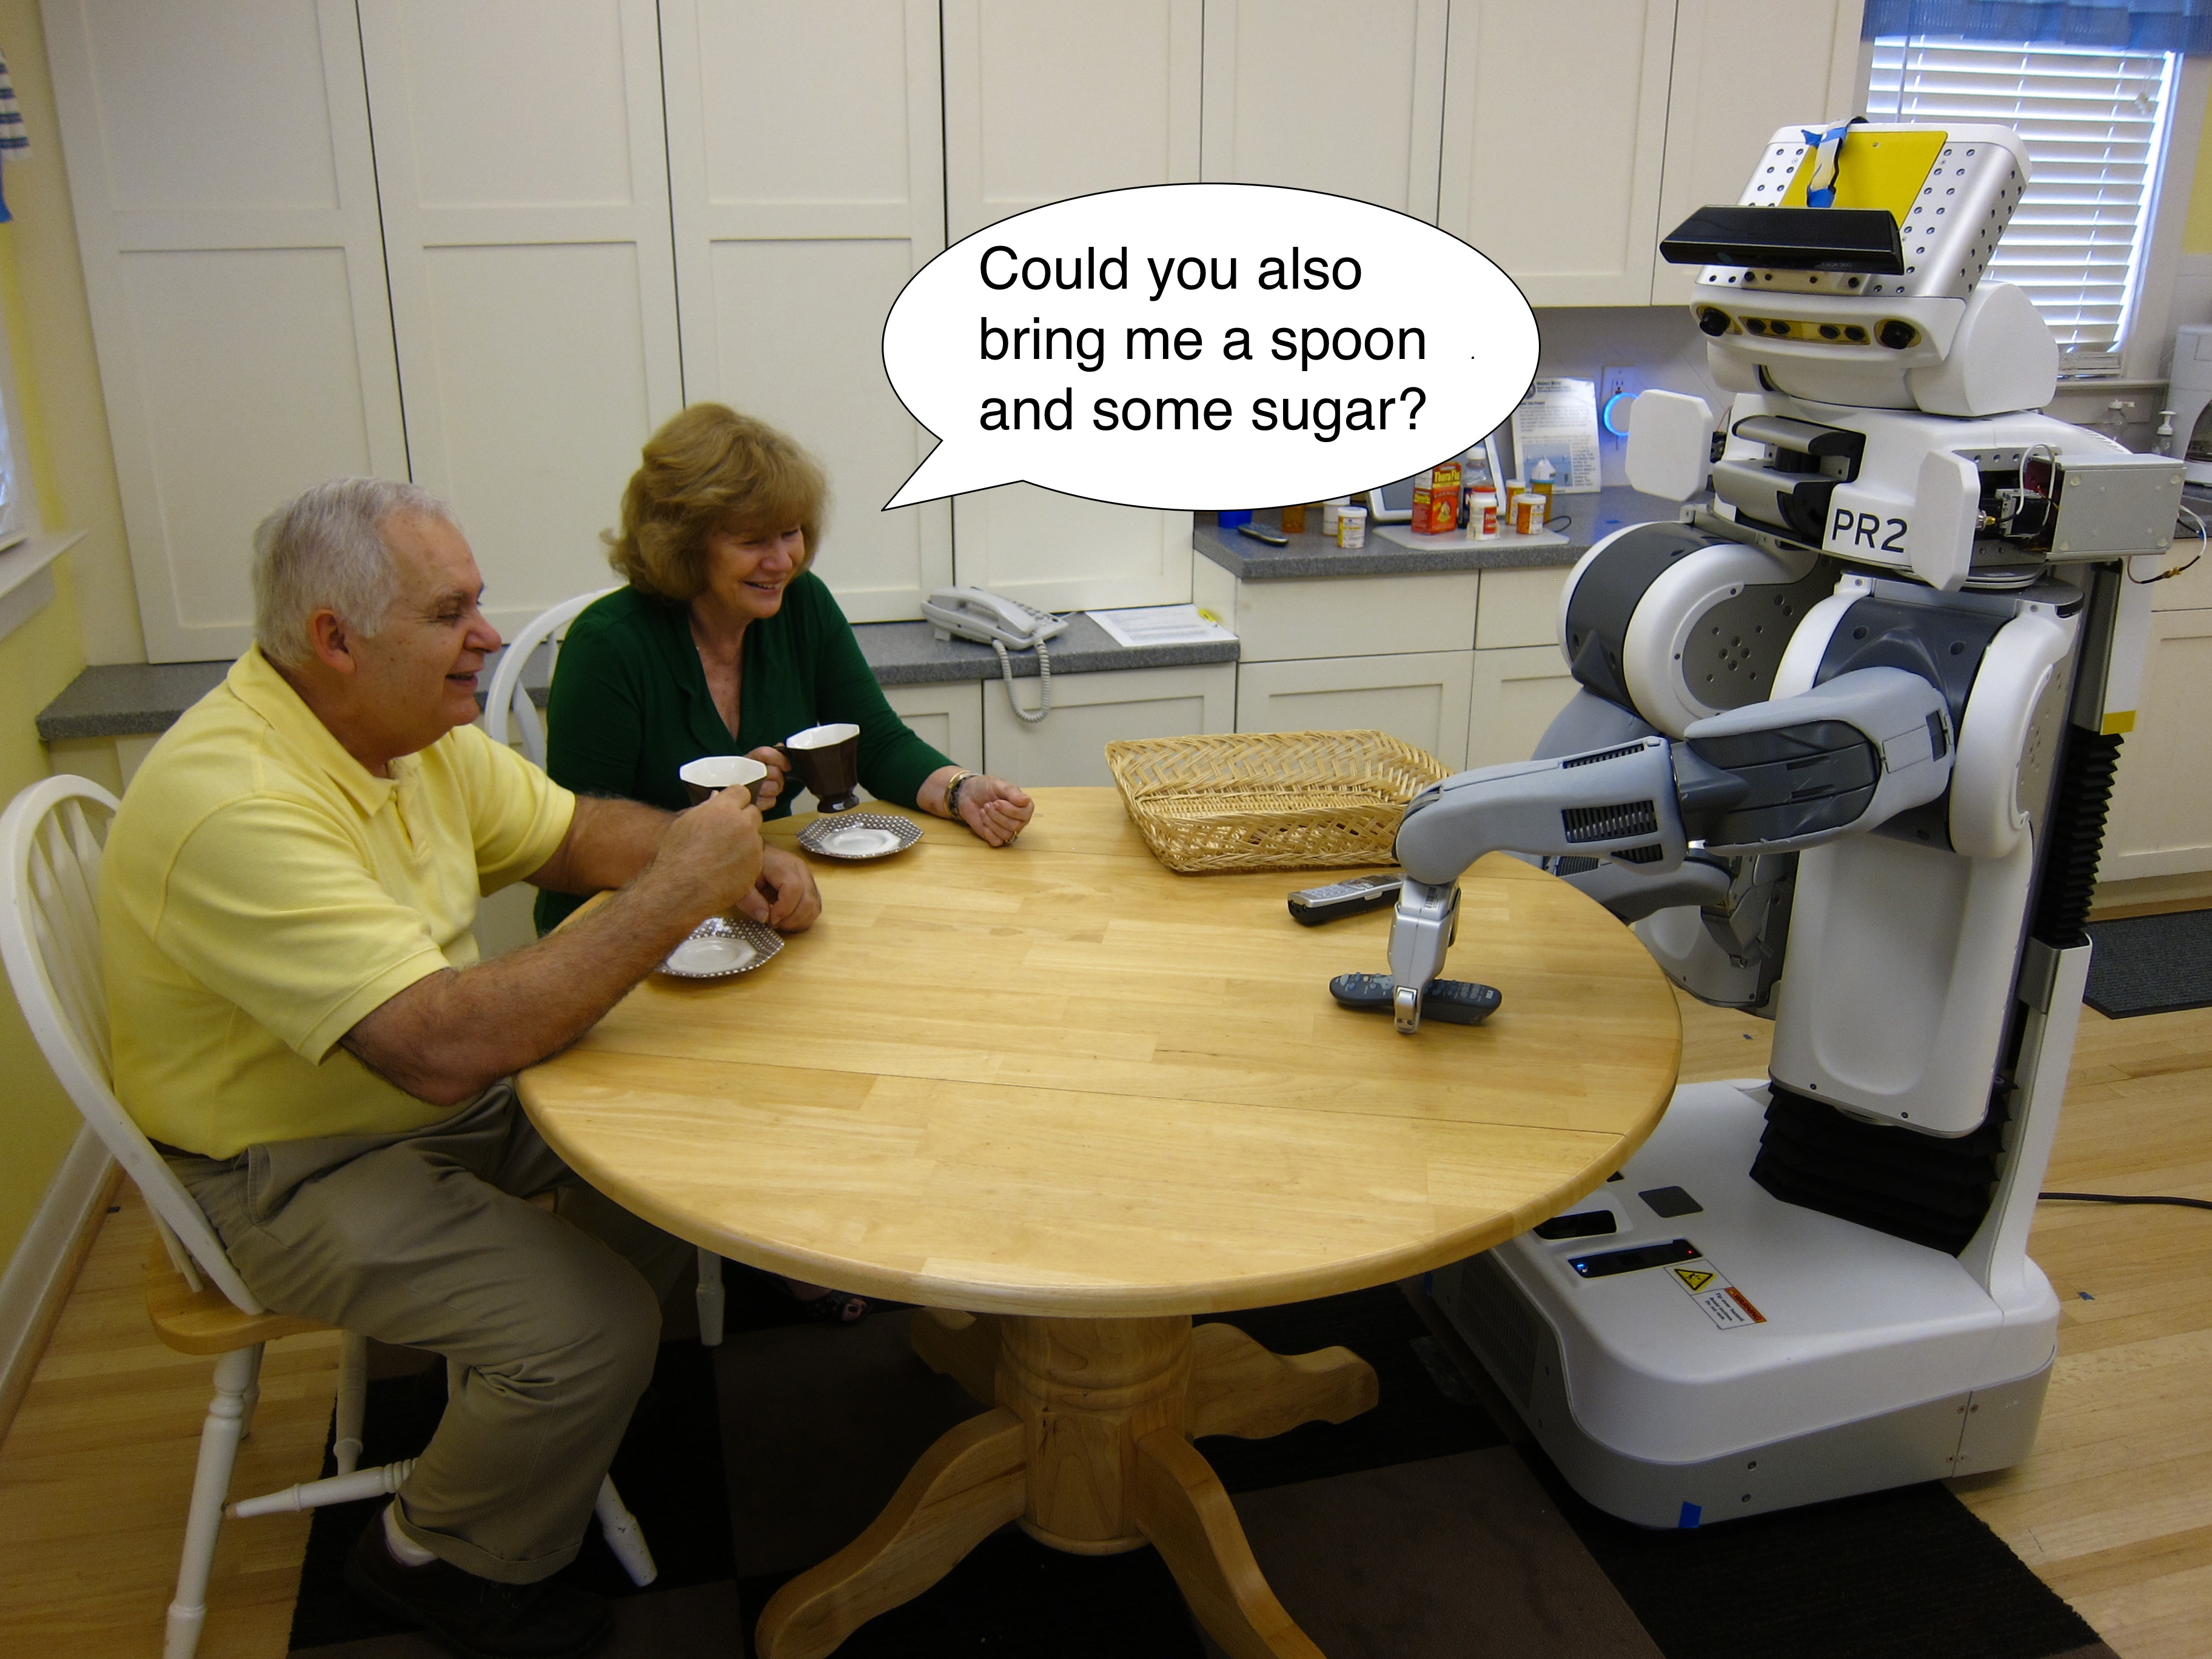
\includegraphics[width=3.2in]{img/robot_in_kitchen.jpg}

    \tiny{Original image courtesy of Wendy Rogers/Georgia Tech}
  \end{center}
\end{frame}

\begin{frame}
  \frametitle{The necessity of manipulation-based search}
  \begin{center}
    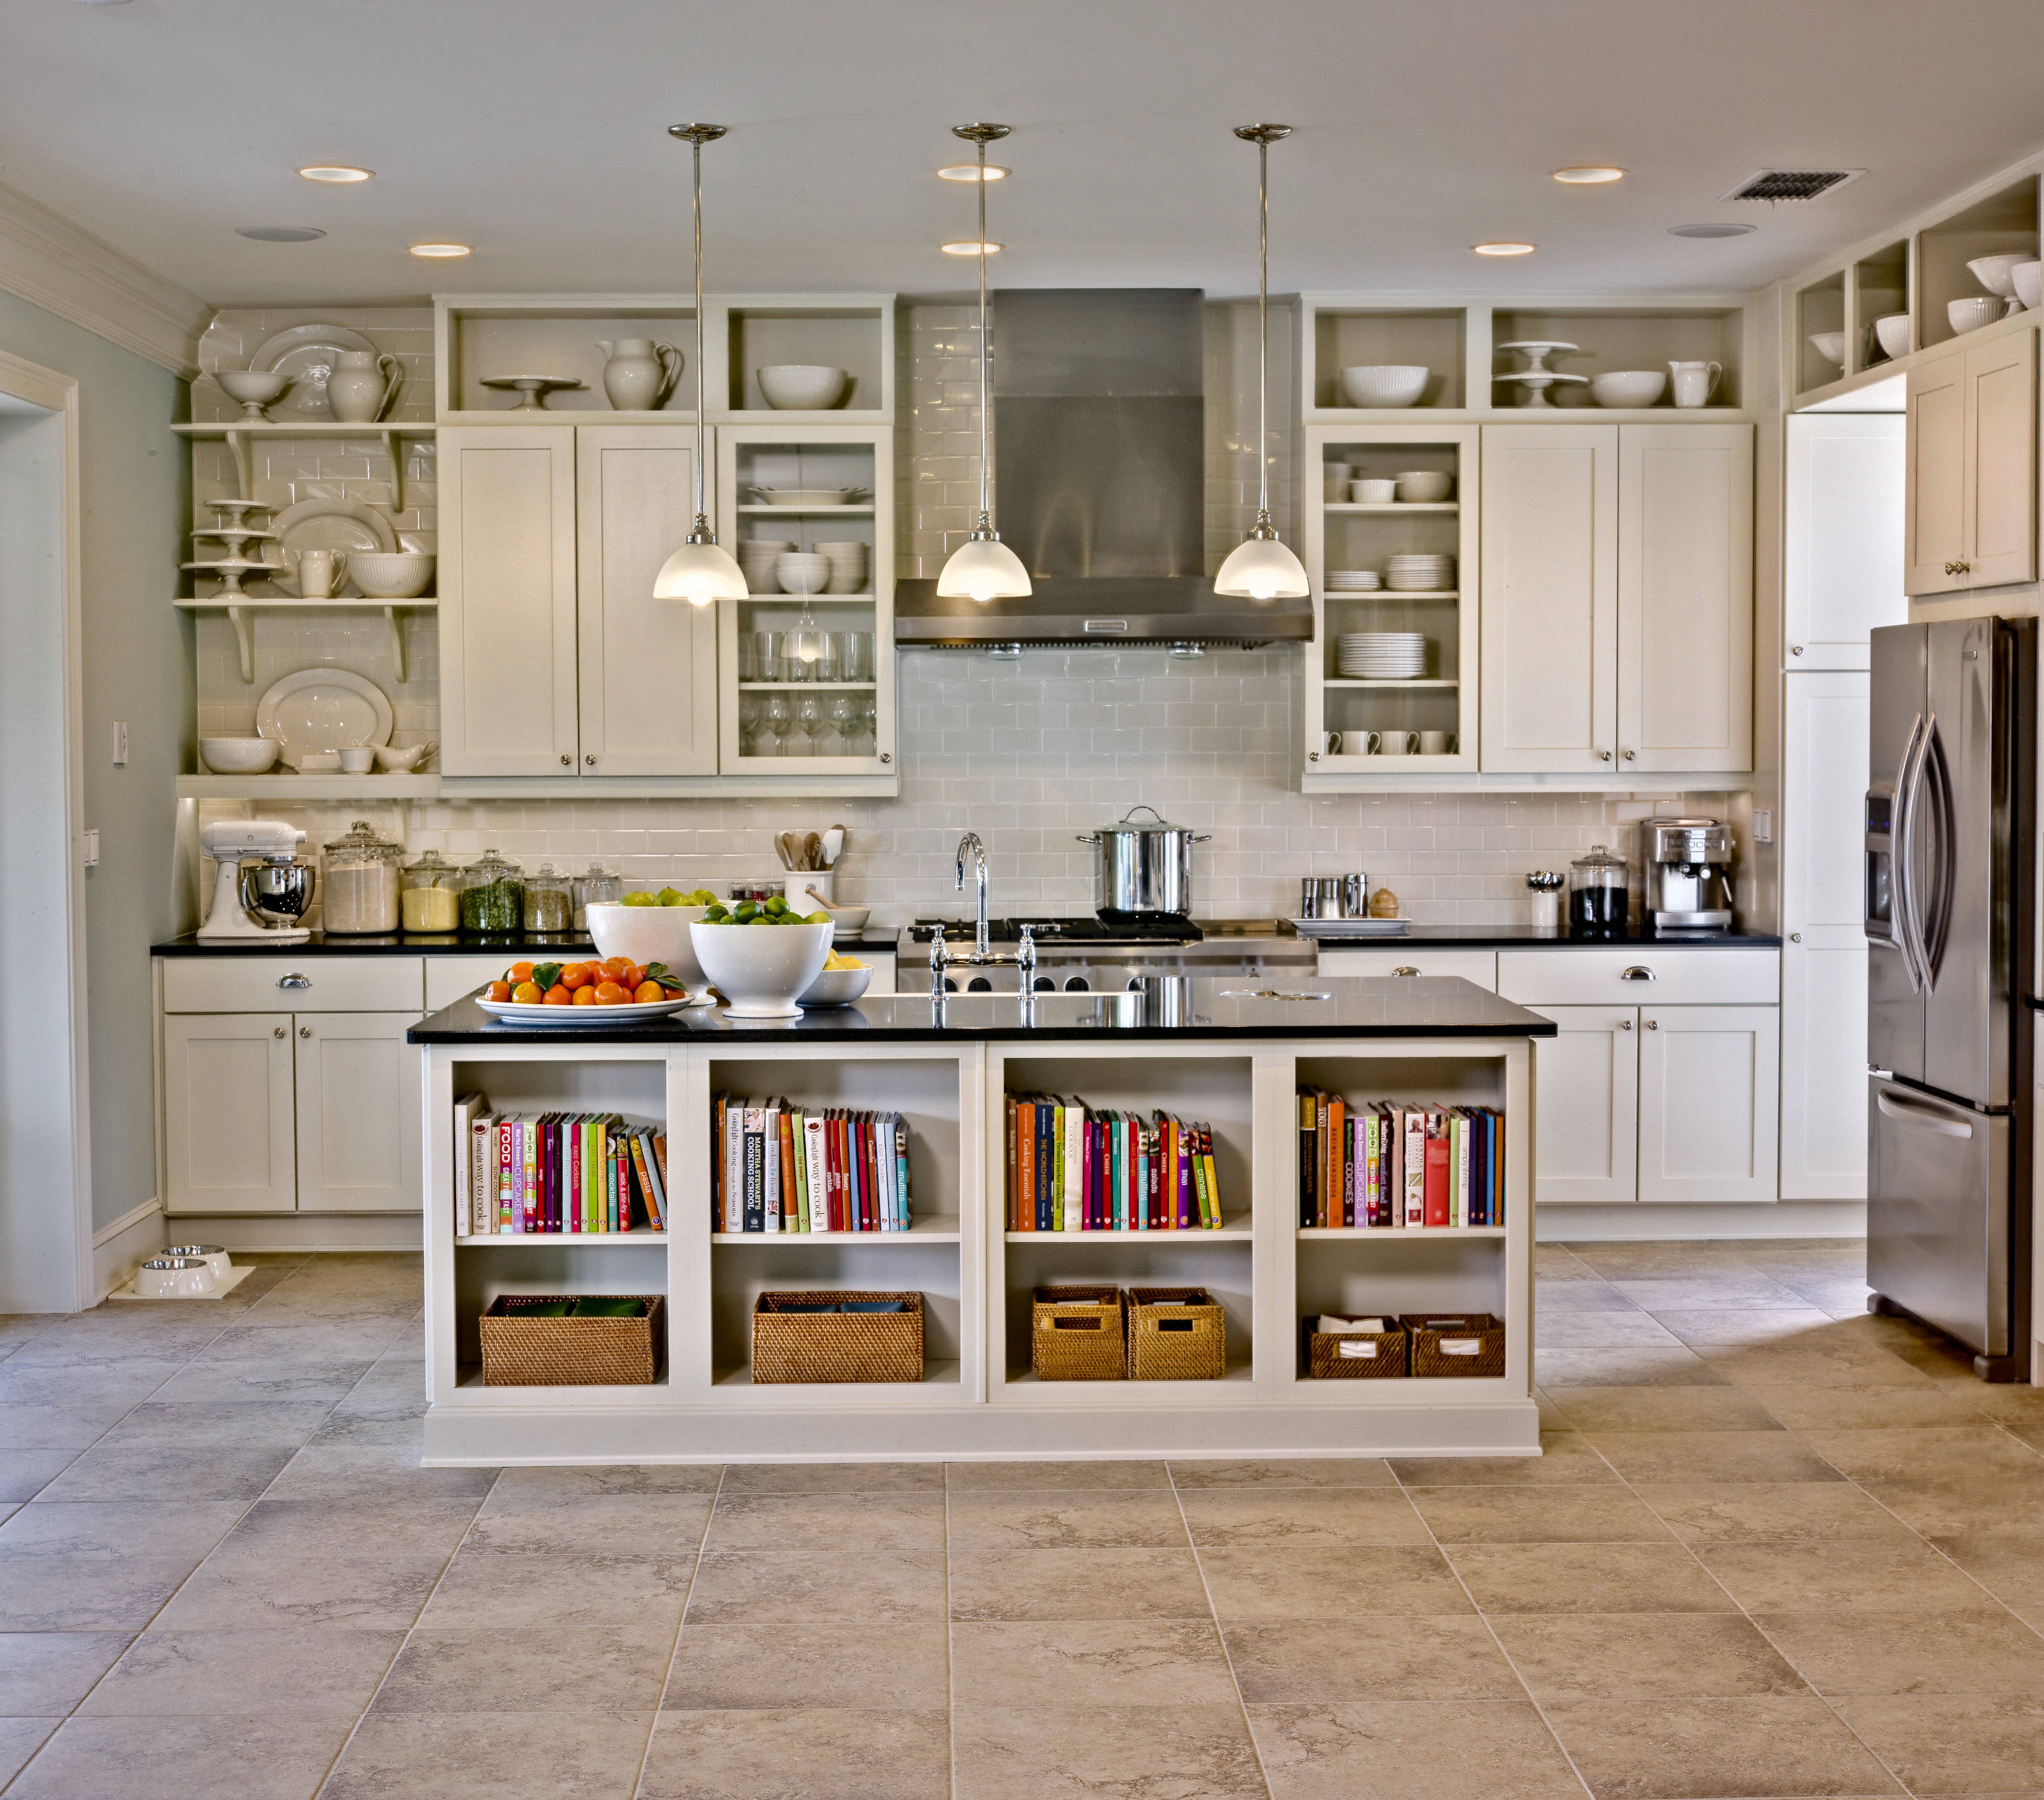
\includegraphics[height=2.7in]{img/kitchen-organization-fake.jpg}

    \tiny{Original image courtesy of personalorganizing.about.com}
  \end{center}
\end{frame}

\begin{frame}
  \frametitle{The necessity of manipulation-based search}
  \vspace{-0.3in}
  \begin{columns}
    \begin{column}{0.6\textwidth}
      \begin{itemize}
        \item Some things are hidden behind other things.
        \item We have to remove items in front to see items in back.
        \item The cookie tray and the rat poison are not likely to be on the same shelf.
      \end{itemize}
    \end{column}
    \begin{column}{0.4\textwidth}
      \begin{center}
        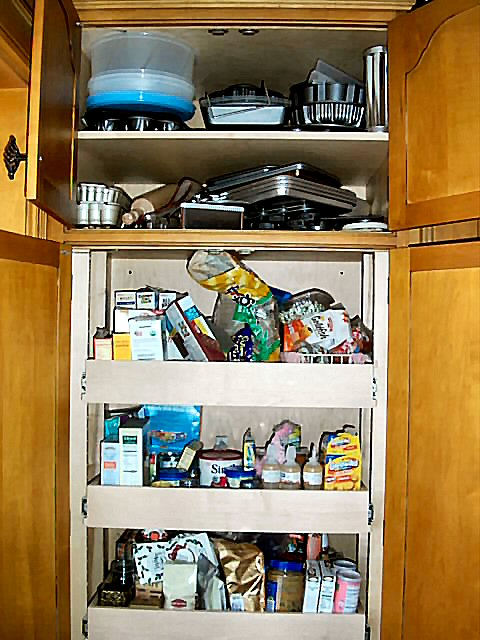
\includegraphics[height=2.7in]{img/kitchen-organization.jpg}

        \tiny{Original image courtesy of shilloh.com}
      \end{center}
    \end{column}
  \end{columns}
\end{frame}

\begin{frame}
  \frametitle{Assumptions for the following treatment}
  \begin{itemize}
  \item No errors in  visual identification and classification of objects
  \item Robot can successfully complete any movement and manipulation task, but
    these are temporally expensive
  \item Finite set of object types in the world
  \end{itemize}
\end{frame}
